\documentclass{beamer}

\synctex=1

\mode<presentation>
{
  \usetheme{Warsaw}
  \setbeamercovered{transparent}
}

\setbeamertemplate{navigation symbols}{}

\graphicspath{ {./images/} }

\setbeamertemplate{footline}
{
  \hfill
  \usebeamercolor[fg]{page number in head/foot}
  \usebeamerfont{page number in head/foot}
  \insertpagenumber\,/\,\insertpresentationendpage\kern1em\vskip2pt
  \leavevmode
  \hbox{\begin{beamercolorbox}[wd=.5\paperwidth,ht=2.5ex,dp=1.125ex,leftskip=.3cm plus1fill,rightskip=.3cm]{author in head/foot}
    \usebeamerfont{author in head/foot}\insertshortauthor
  \end{beamercolorbox}
  \begin{beamercolorbox}[wd=.5\paperwidth,ht=2.5ex,dp=1.125ex,leftskip=.3cm,rightskip=.3cm plus1fil]{title in head/foot}
    
    \usebeamerfont{title in head/foot}\insertshorttitle
  \end{beamercolorbox}}
  \vskip0pt
}

\usepackage[british]{babel}
\usepackage{times}
\usepackage[latin1]{inputenc}
\usepackage[T1]{fontenc}
\usepackage{lmodern}
\usepackage{amsmath,amsthm,amssymb}
\usepackage{hyperref}
\usepackage{nccfoots}

%\newtheorem{definition}{Definition}
%\newtheorem{theorem}{Theorem}
\newtheorem{conjecture}{Conjecture}

\renewcommand{\t}{$\mathrm{t}$}
\newcommand{\BHV}{$\mathrm{BHV}$}
\newcommand{\NP}{$\mathrm{NP}$}
\newcommand{\MCMC}{$\mathrm{MCMC}$}
\newcommand{\SPR}{$\mathrm{SPR}$}

\title[Portobello `15: {\em The space of ultrametric phylogenetic trees}]{The space of ultrametric phylogenetic trees}

\author[Gavryushkin-Drummond ~~~~~~~~~~~~~ \href{mailto:a.gavruskin@auckland.ac.nz}{a.gavruskin@auckland.ac.nz}]{Alex Gavryushkin\\ (joint work with Alexei Drummond) \\ \ \\

\includegraphics[height=2cm]{UniAuckland}}

\date{2nd February 2015}

\begin{document}
%%%%%%%%%%%%%%%%%%%%%%%%%%%%%%%%%%%%%%%%%%%%%%%%%%%%%%%%%%%%%%%%%%%%%%

\begin{frame}
\titlepage
\end{frame}

\begin{frame}{Plan}

\begin{enumerate}
\item Comic definitions 
\item Real definitions (by request)
\item Motivation 
\item Results 
\end{enumerate}
\end{frame}

\begin{frame}{Unrooted phylogenetic tree}

\begin{definition}
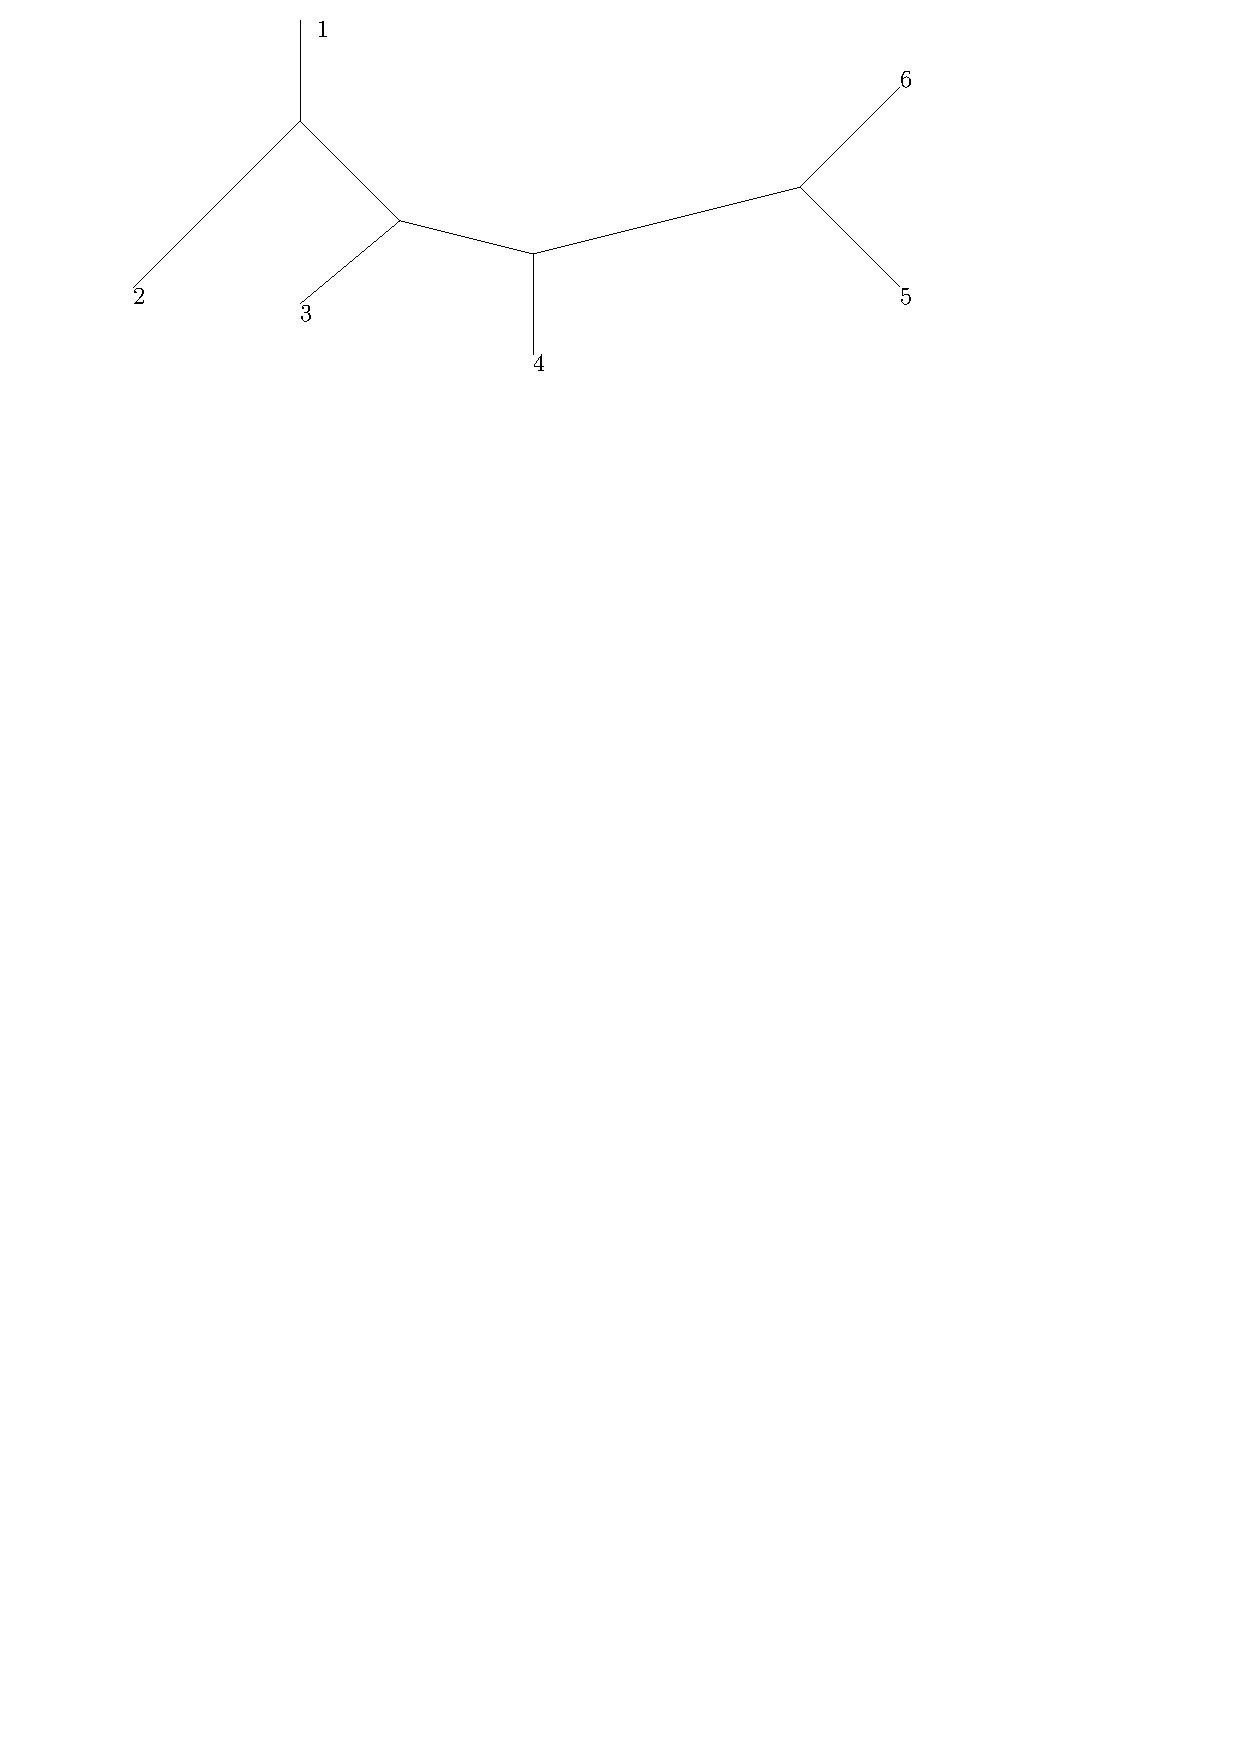
\includegraphics[width=\framewidth]{unrooted}
\end{definition}
\end{frame}

\begin{frame}{Real Life}
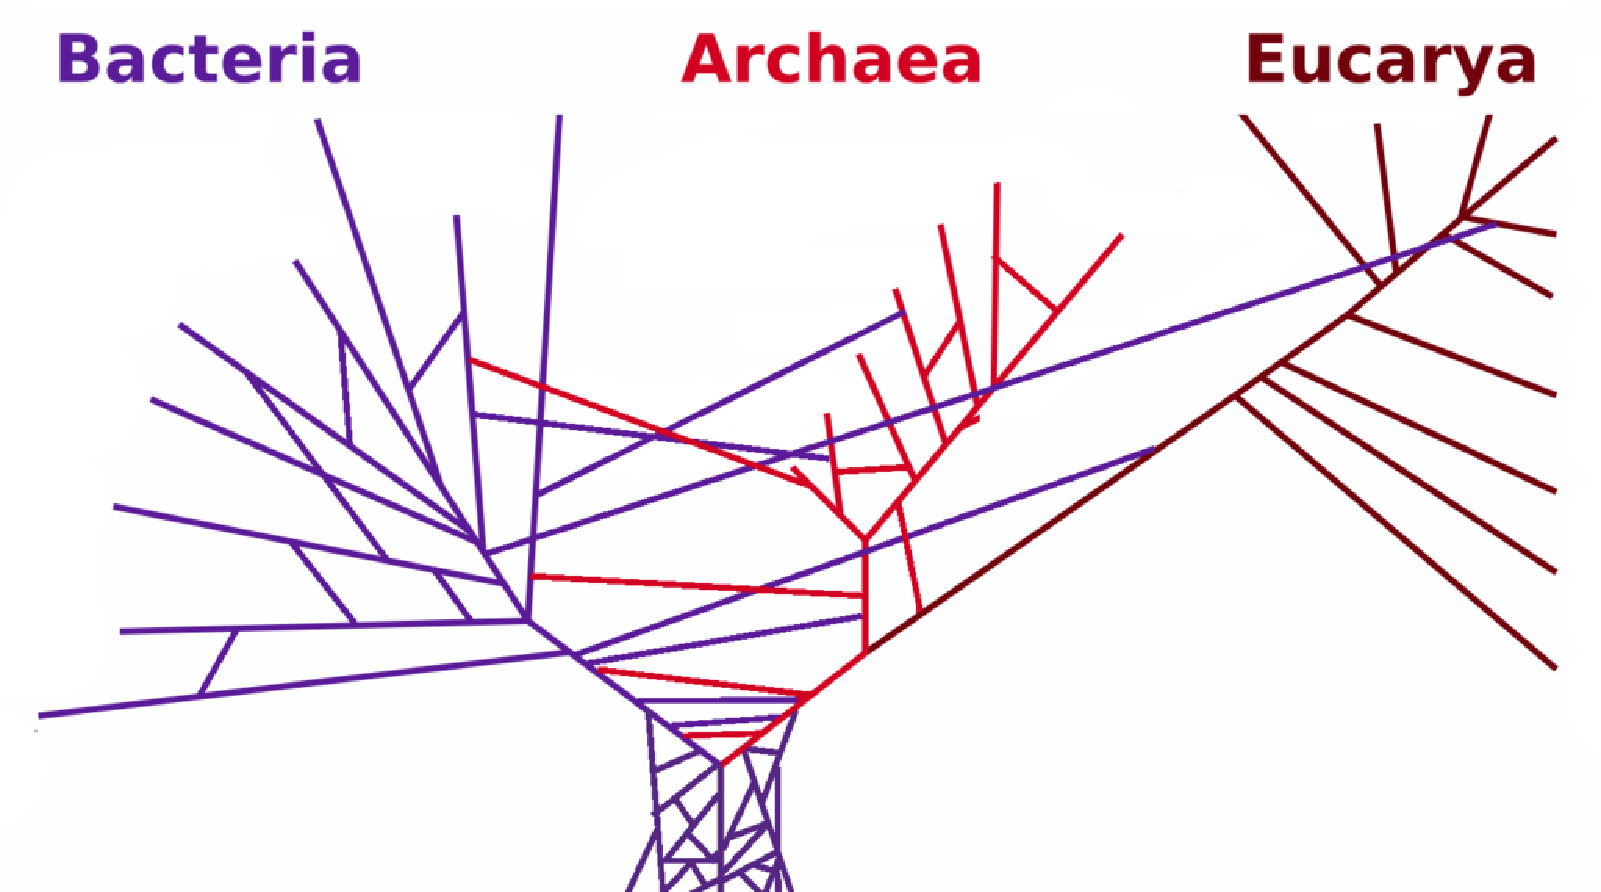
\includegraphics[width=\framewidth]{realLife.pdf}

\vfill

\tiny
Credit link:
\href{http://commons.wikimedia.org/wiki/File:PhylogeneticTree_horizontal_transfers.png?uselang=en-gb}{http://commons.wikimedia.org/wiki/File:PhylogeneticTree\_horizontal\_transfers.png?uselang=en-gb}
\end{frame}

\begin{frame}{Rooted phylogenetic tree}
\begin{definition}
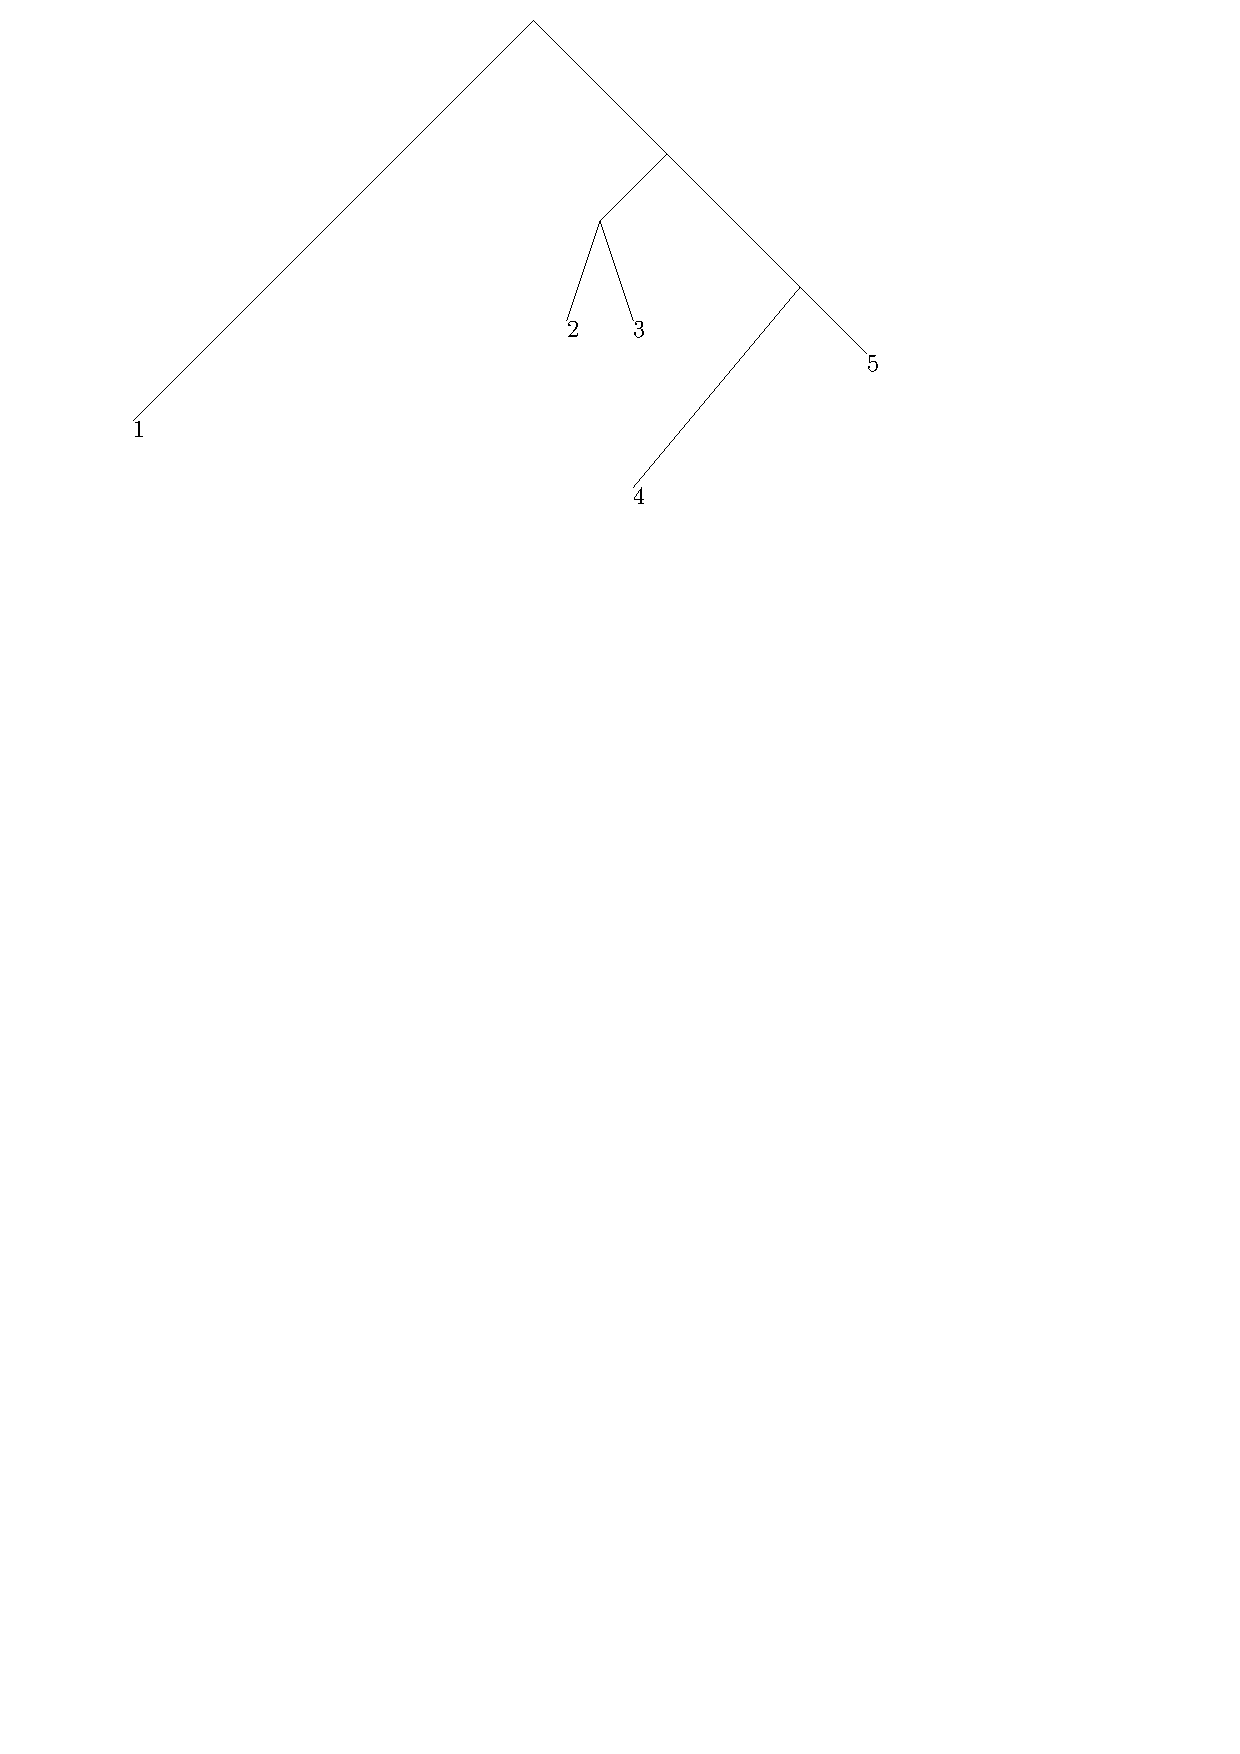
\includegraphics[width=\framewidth]{rooted}
\end{definition}
\end{frame}

\begin{frame}{Equidistant (ultrametric) phylogenetic tree}
\begin{definition}
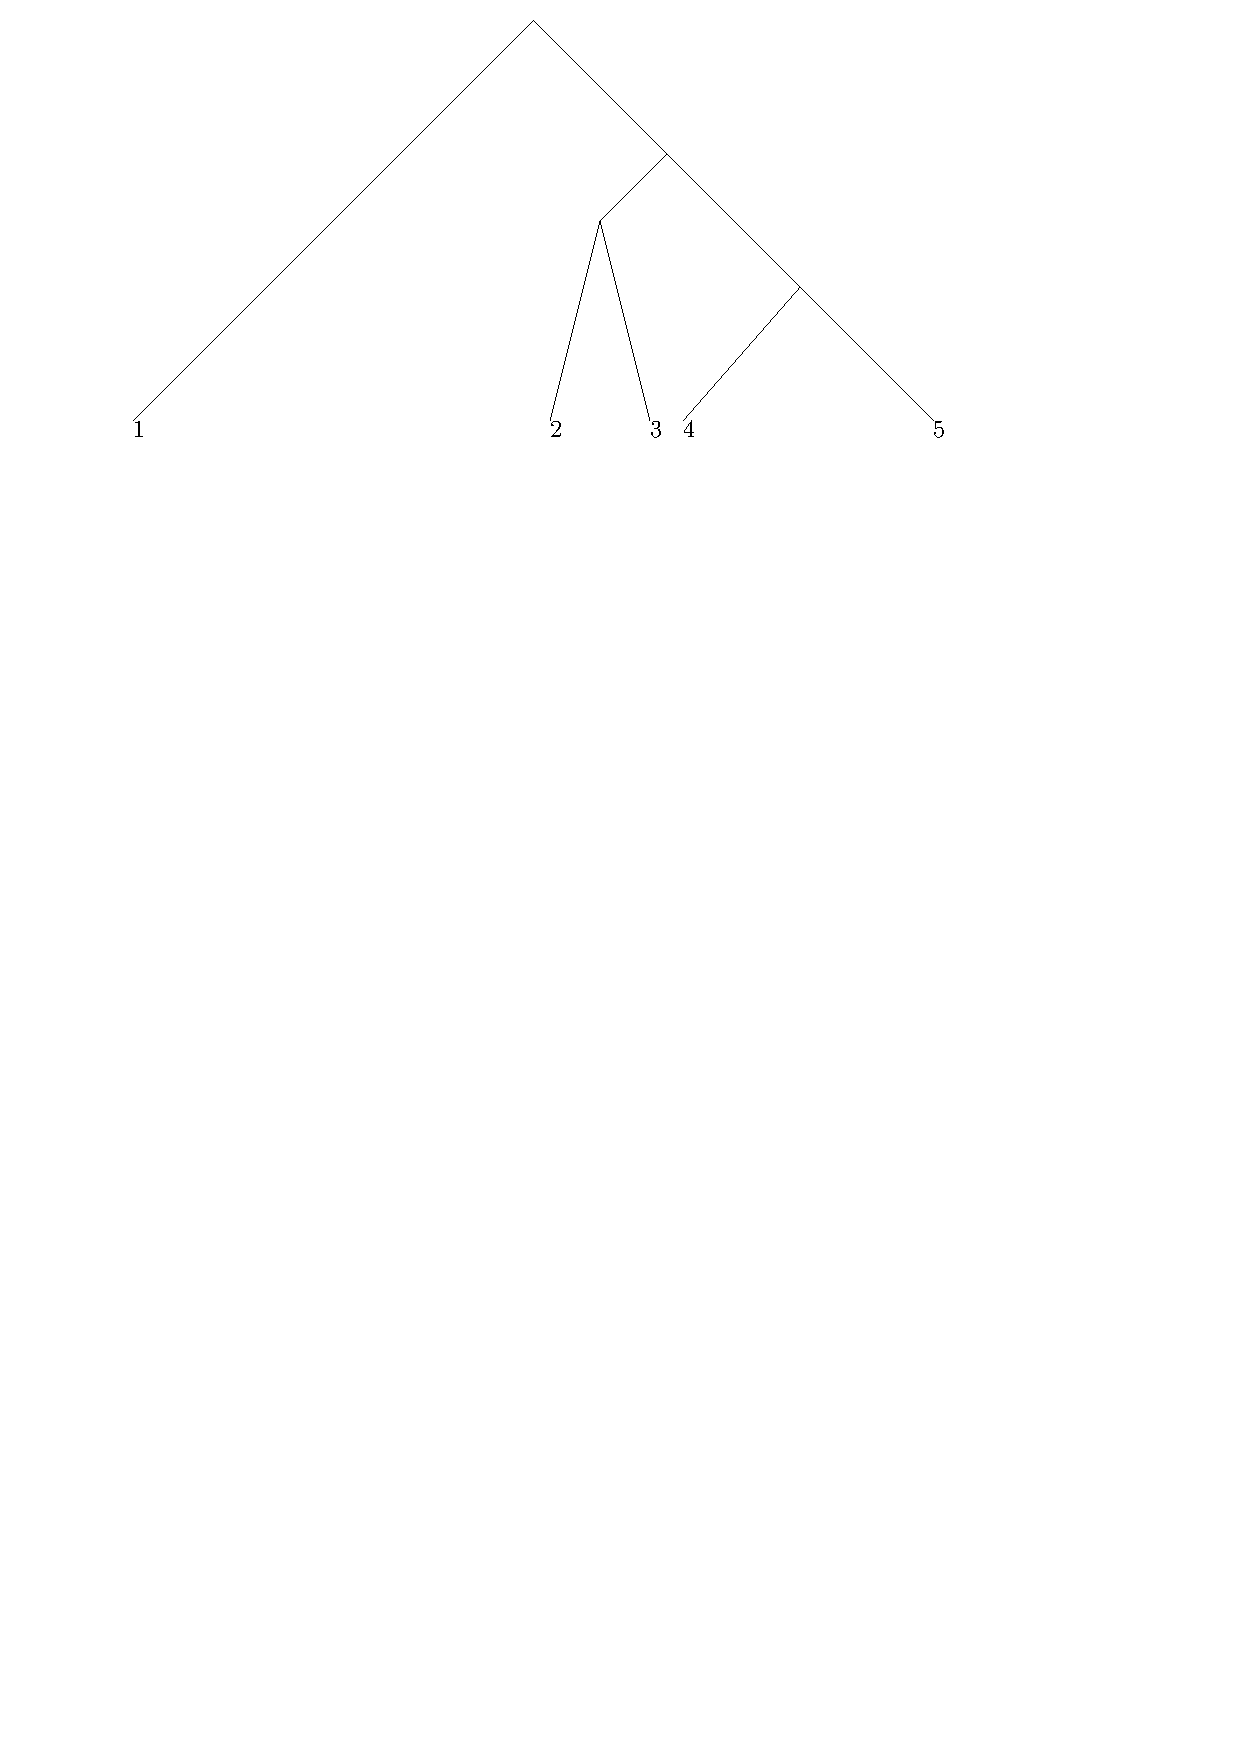
\includegraphics[width=\framewidth]{rooted_time}
\end{definition}
\end{frame}

\begin{frame}{Equidistant phylogenetic tree with parameters}
\begin{definition}
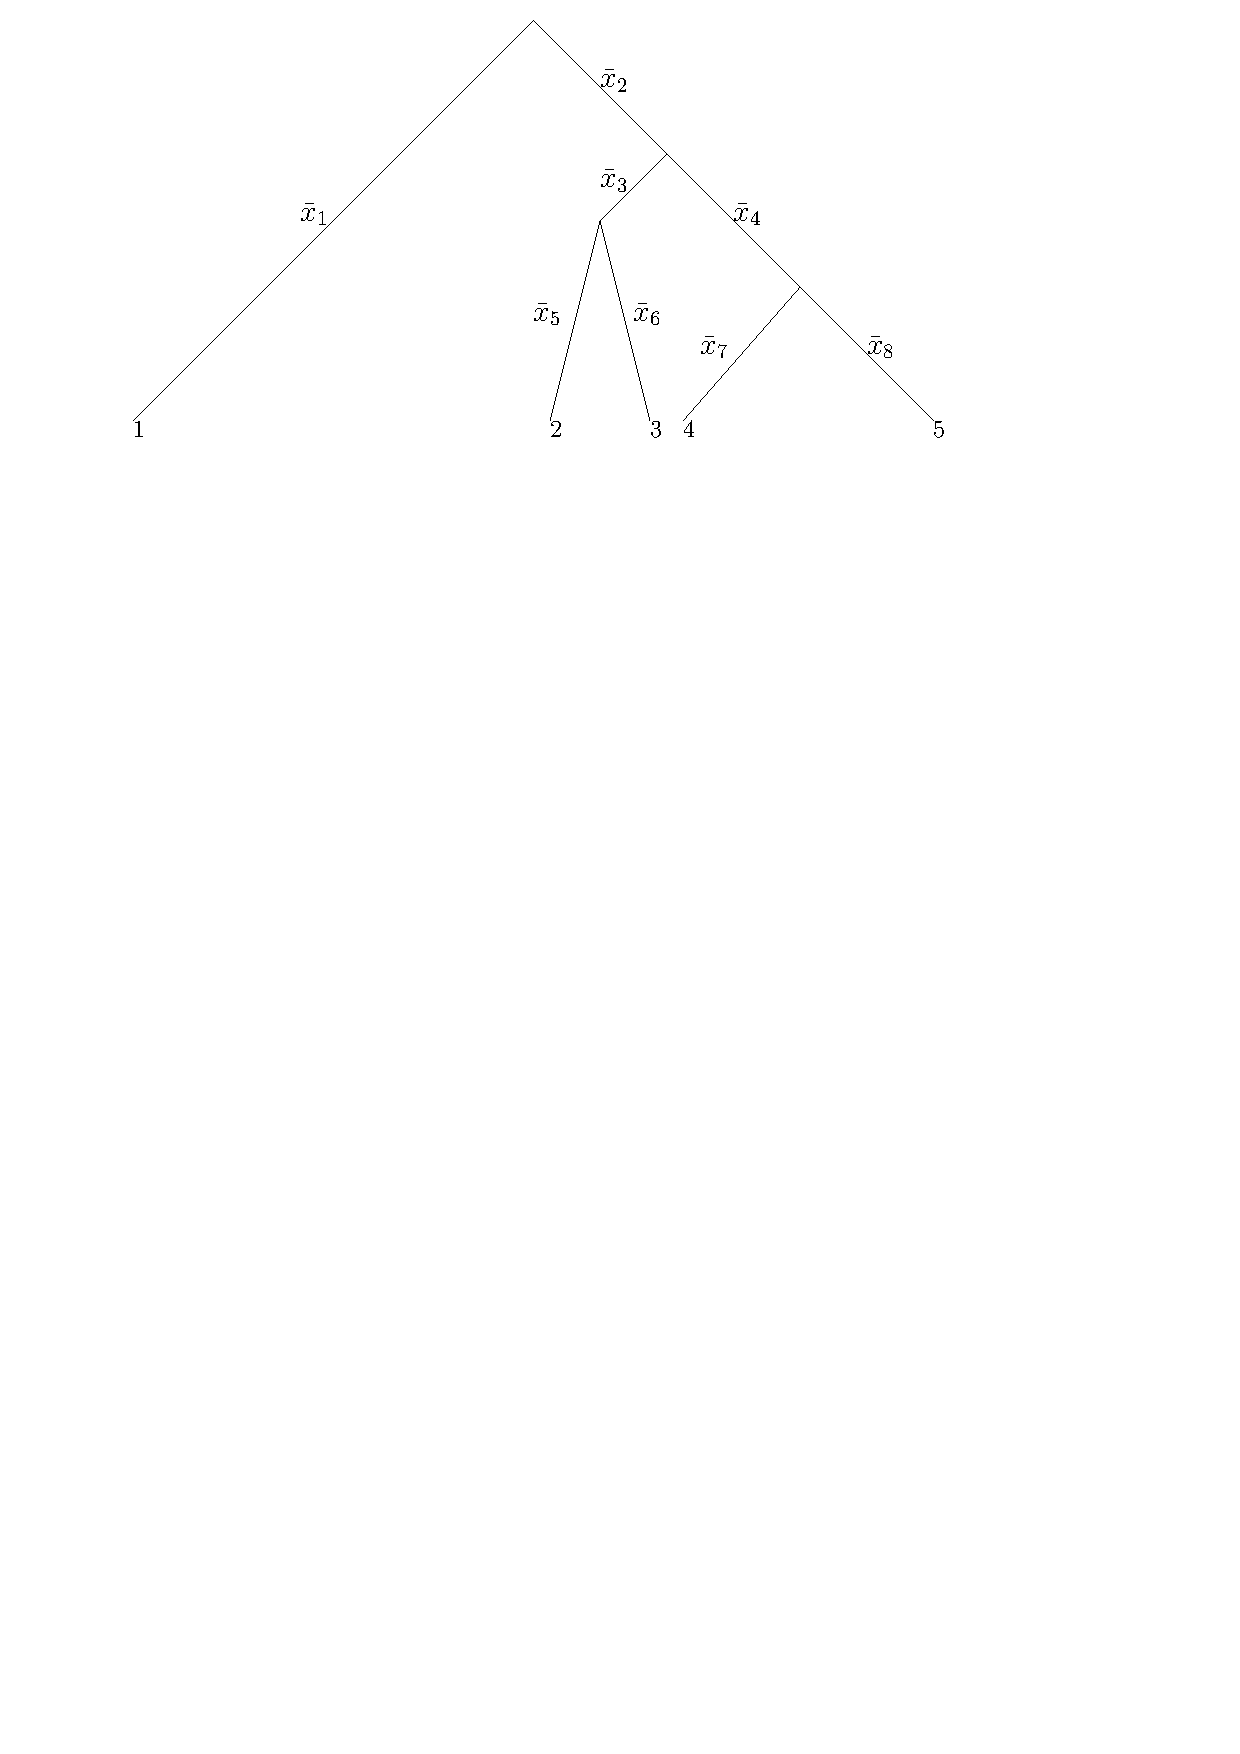
\includegraphics[width=\framewidth]{rooted_time_parameters}
\end{definition}
\end{frame}

\begin{frame}{$\tau$-parameterisation}
\begin{definition}
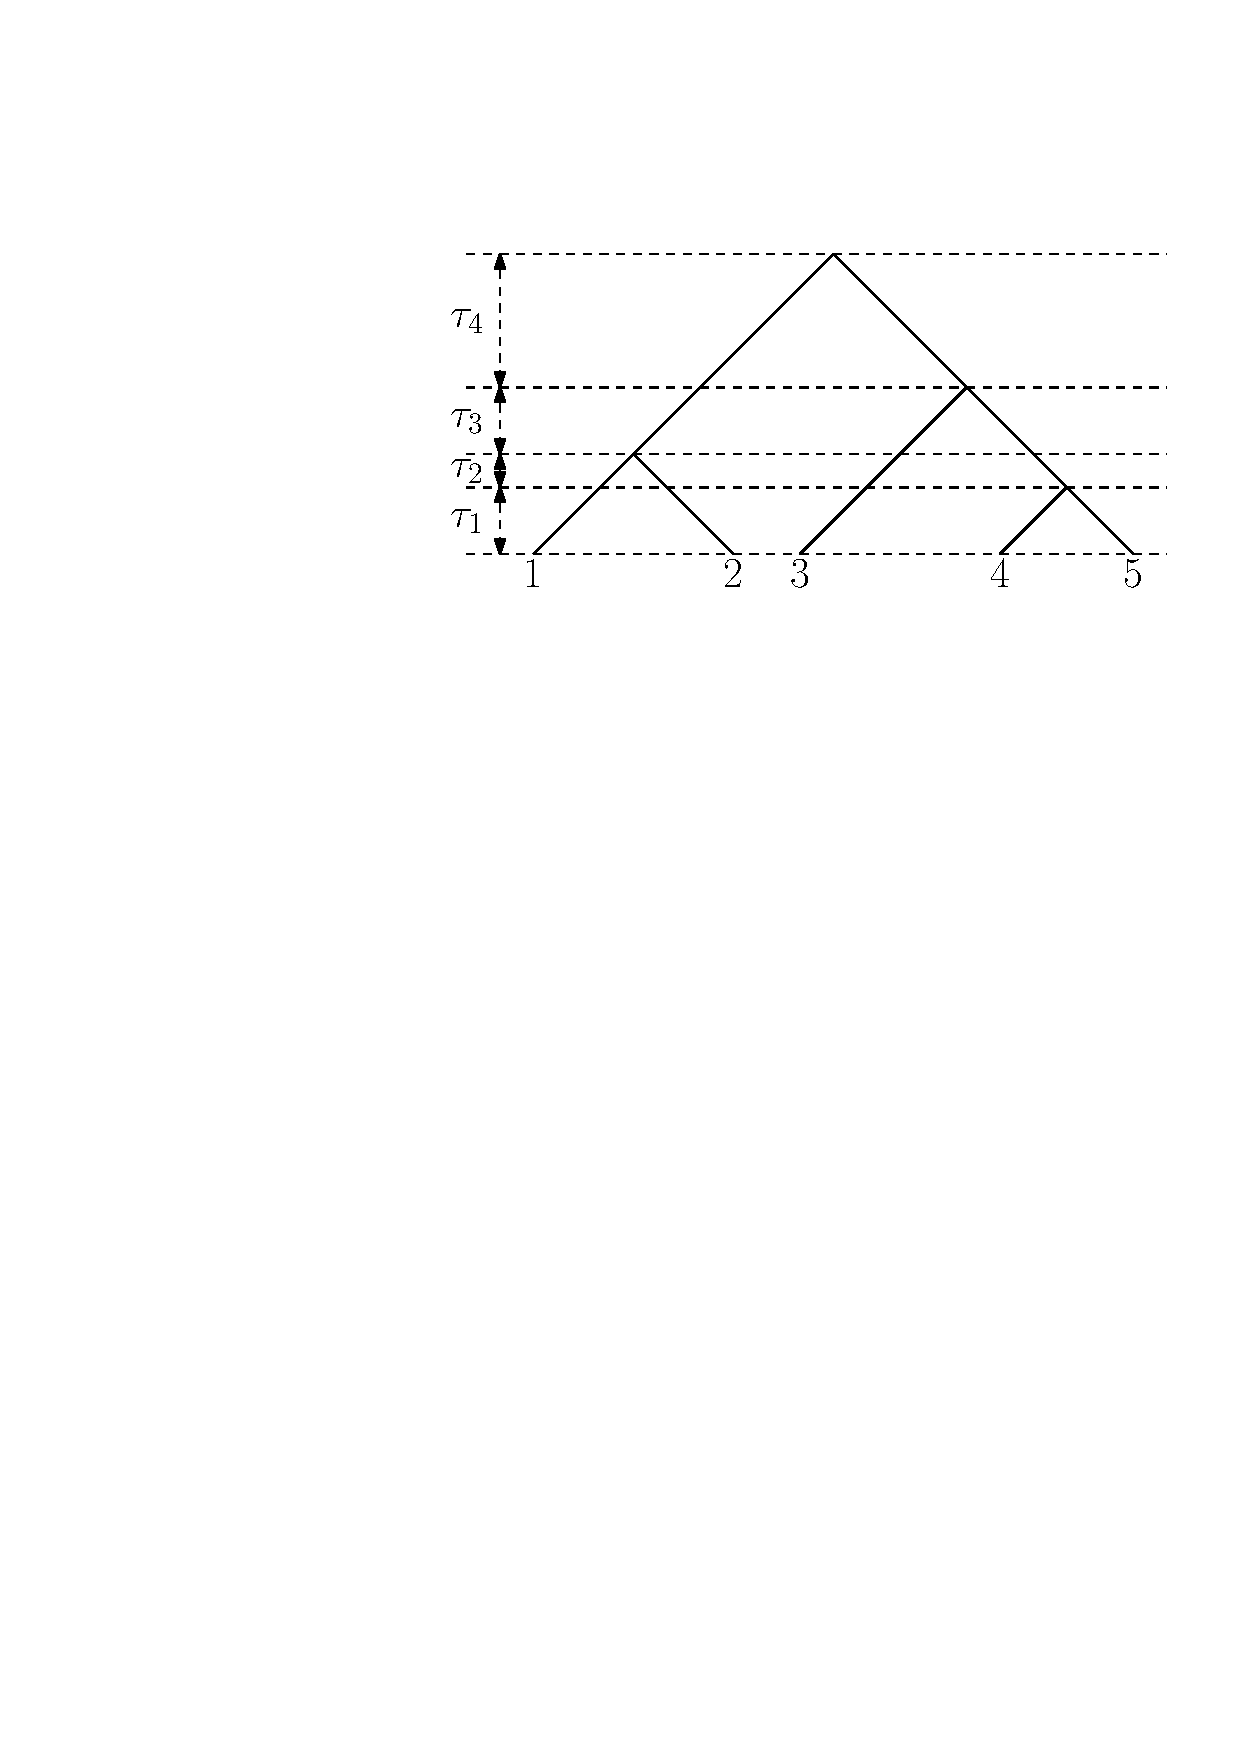
\includegraphics[width=\framewidth]{T5}
\end{definition}
\end{frame}

\begin{frame}{$\tau$-space}
\begin{definition}
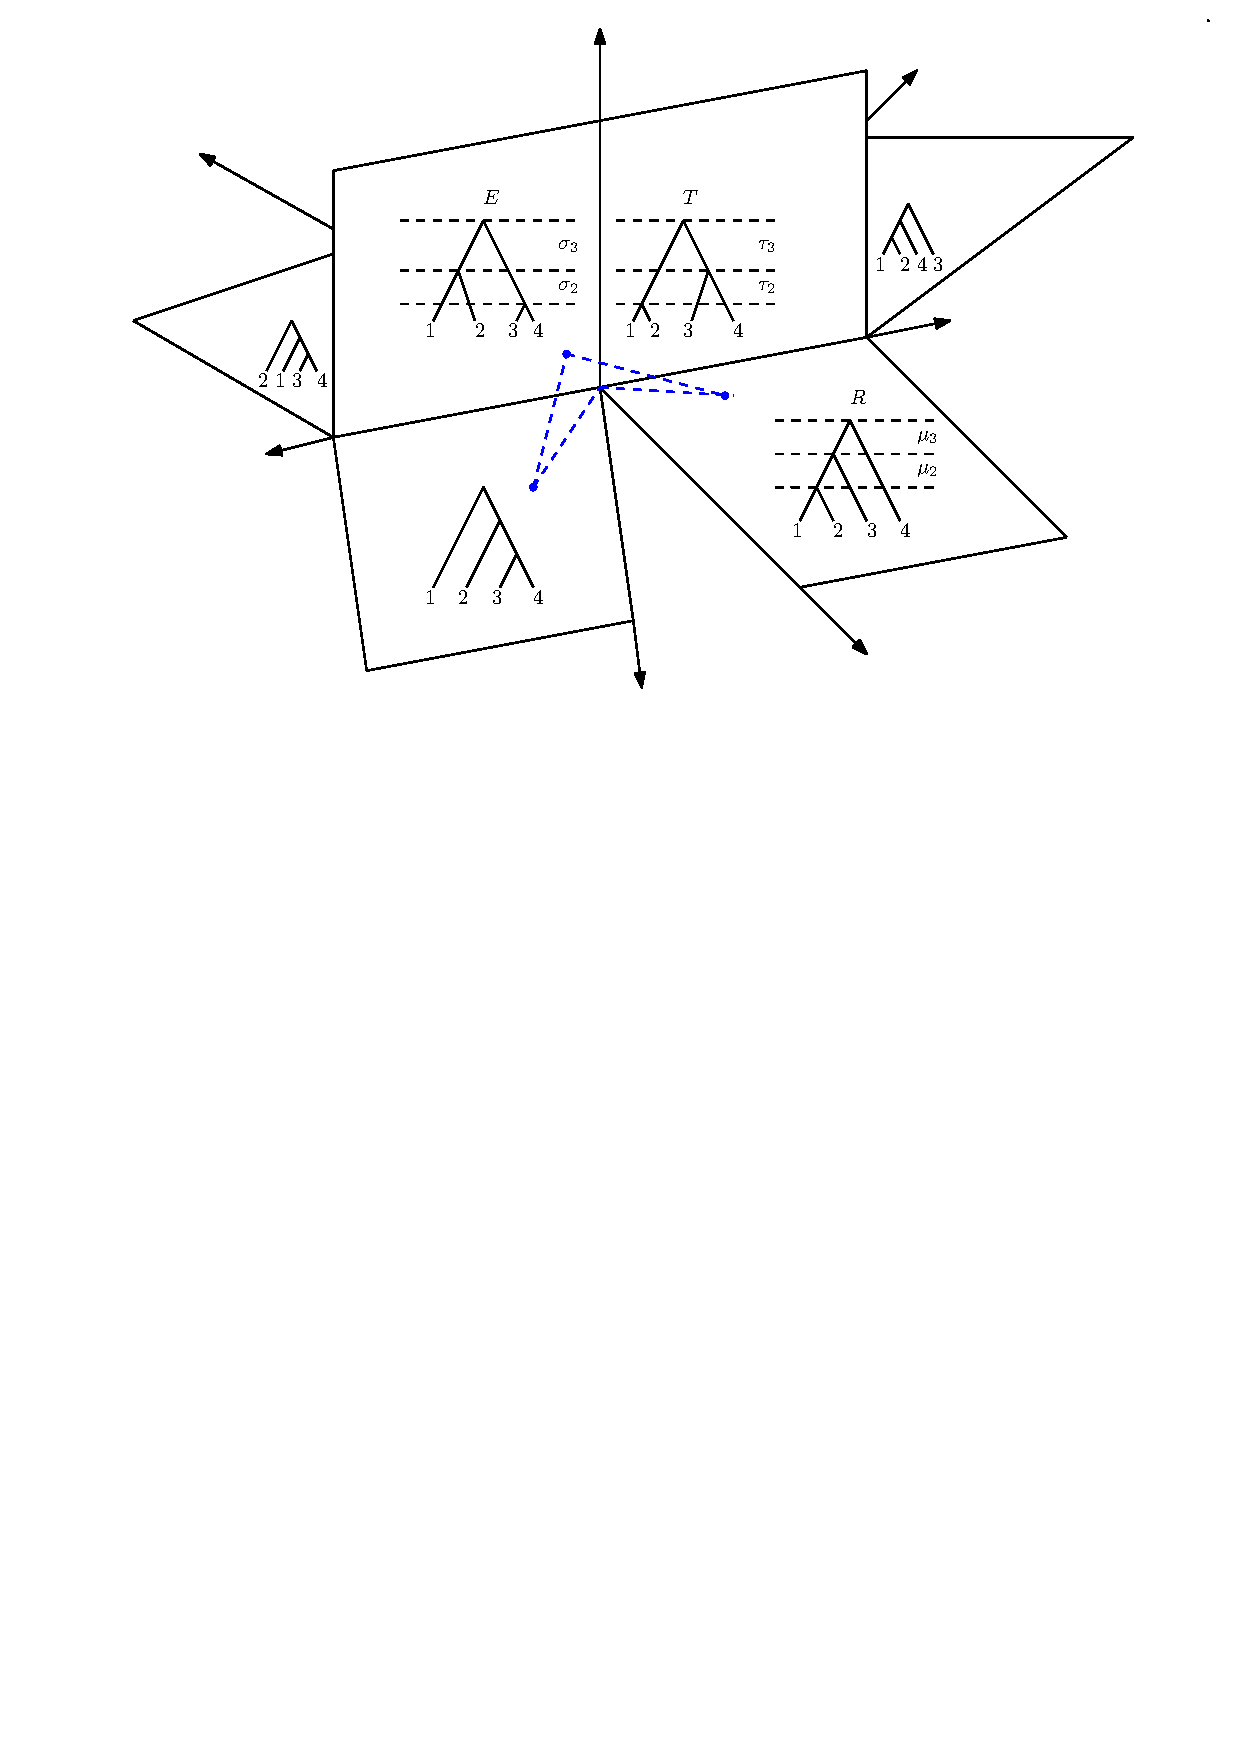
\includegraphics[width=\framewidth]{tauSpace}
\end{definition}
\end{frame}

\begin{frame}{\t-parameterisation}
\begin{definition}
\begin{center}
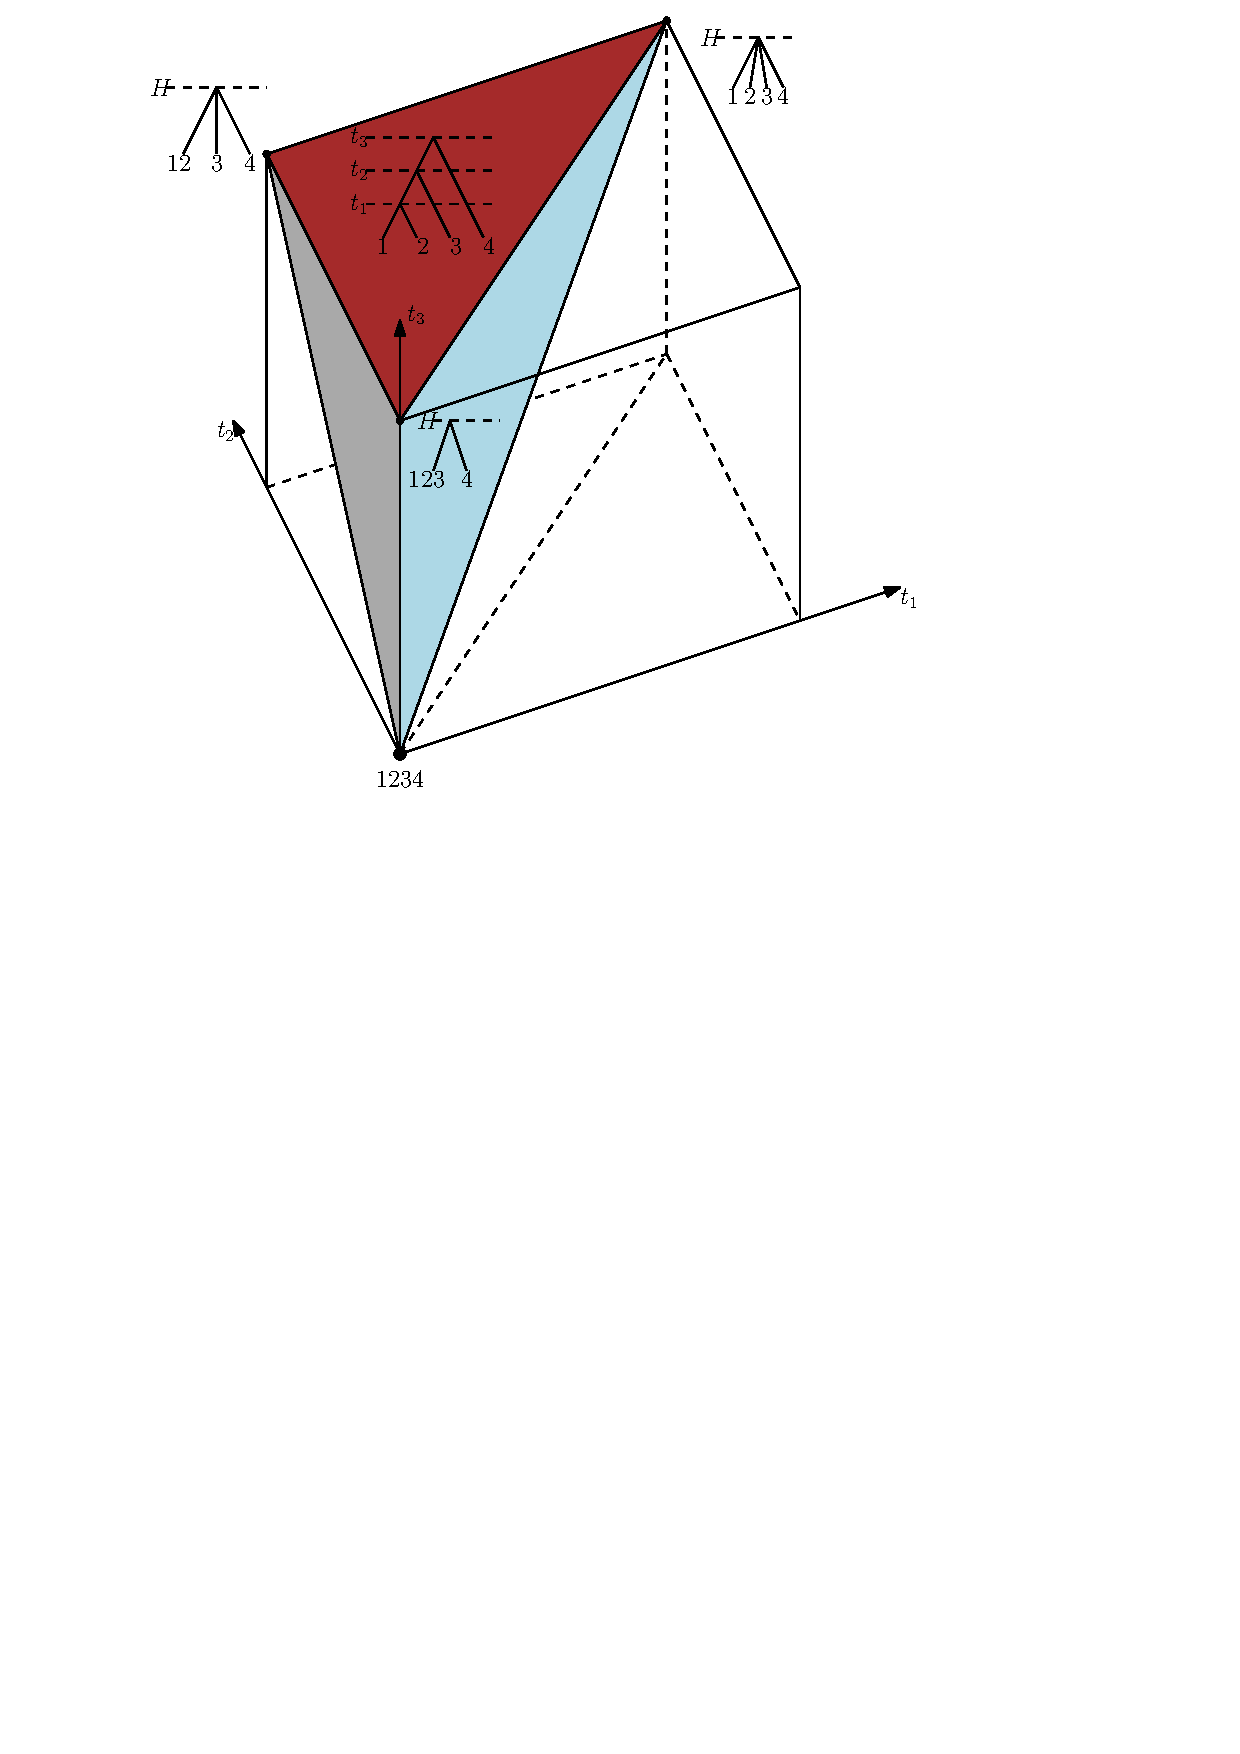
\includegraphics[width=0.65\framewidth]{simplex}
\end{center}
\end{definition}
\end{frame}

\begin{frame}{\t-space}
\begin{definition}
\begin{center}
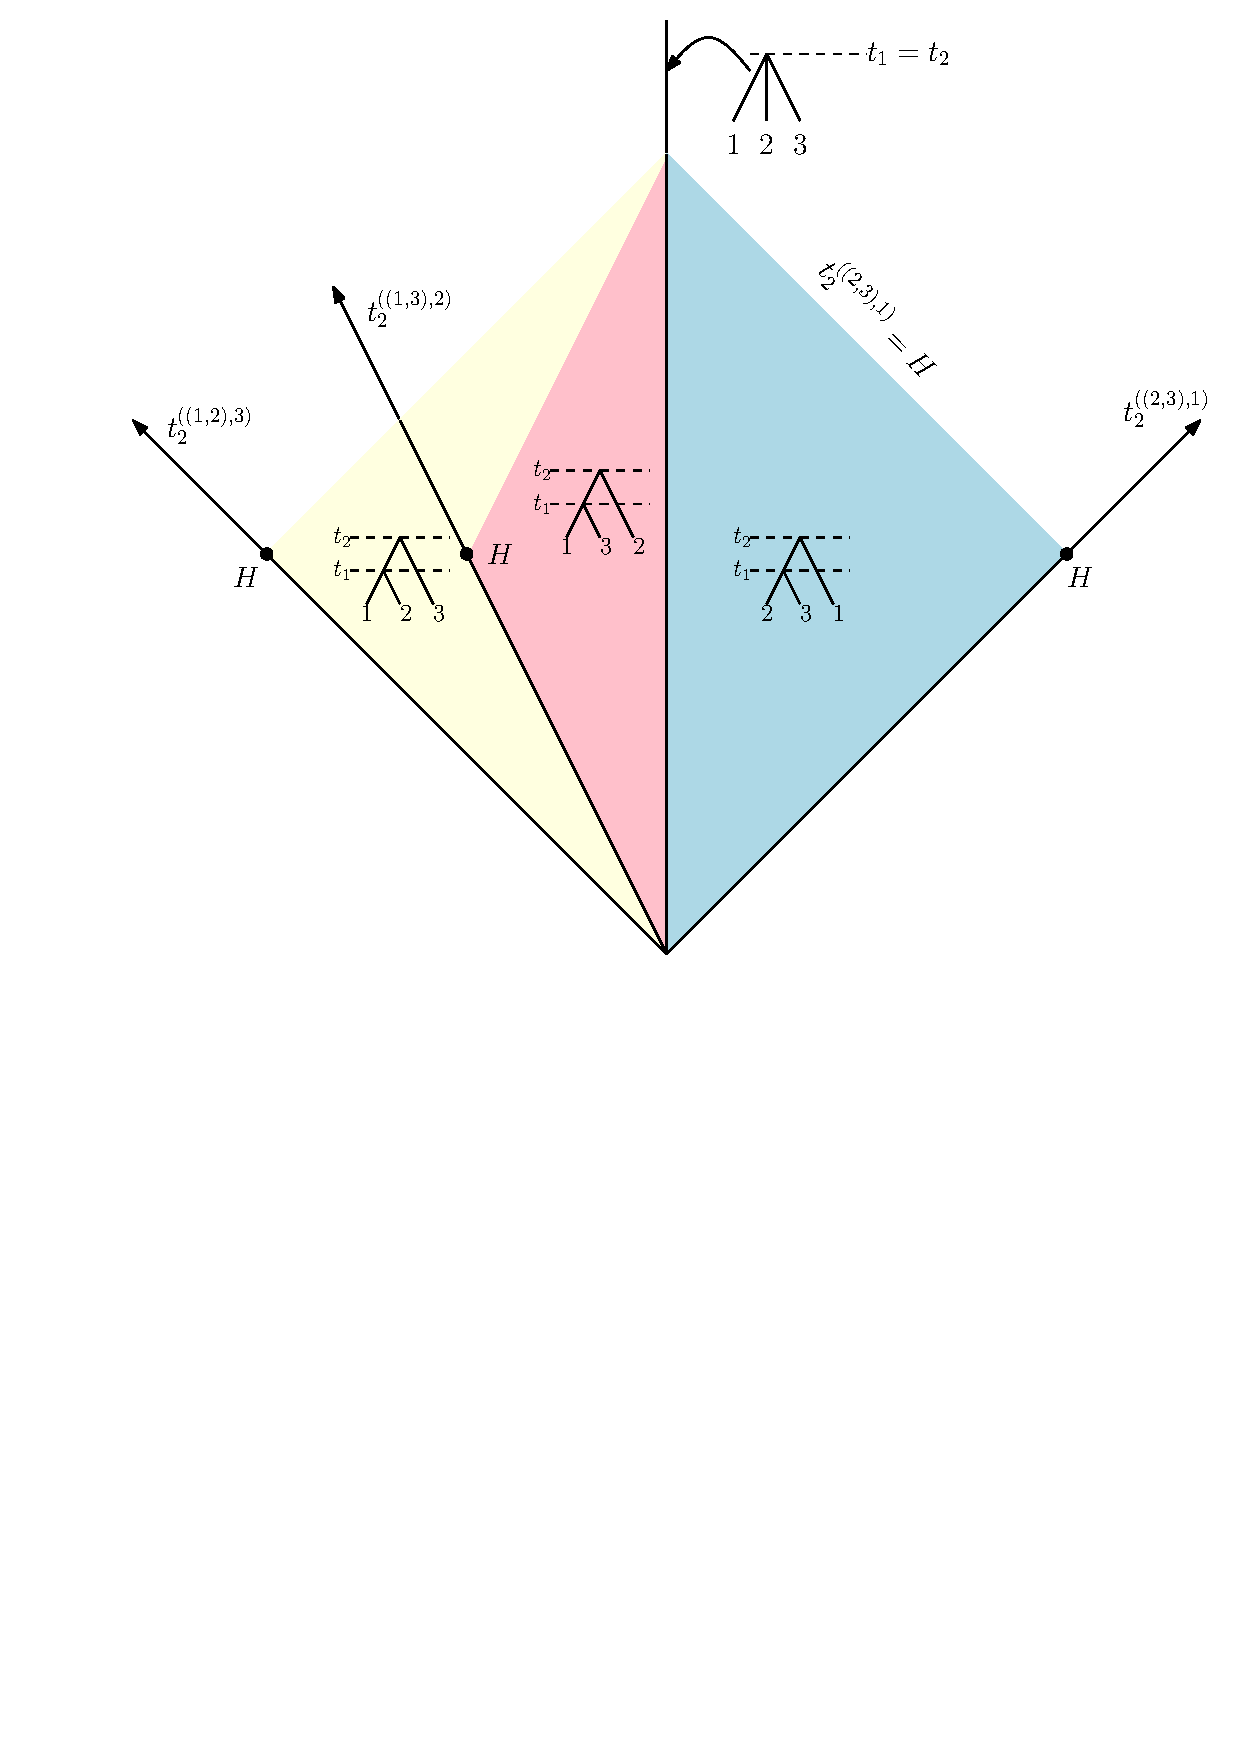
\includegraphics[width=0.78\framewidth]{tSpace2d}
\end{center}
\end{definition}
\end{frame}

\begin{frame}{\t-space}
\begin{definition}
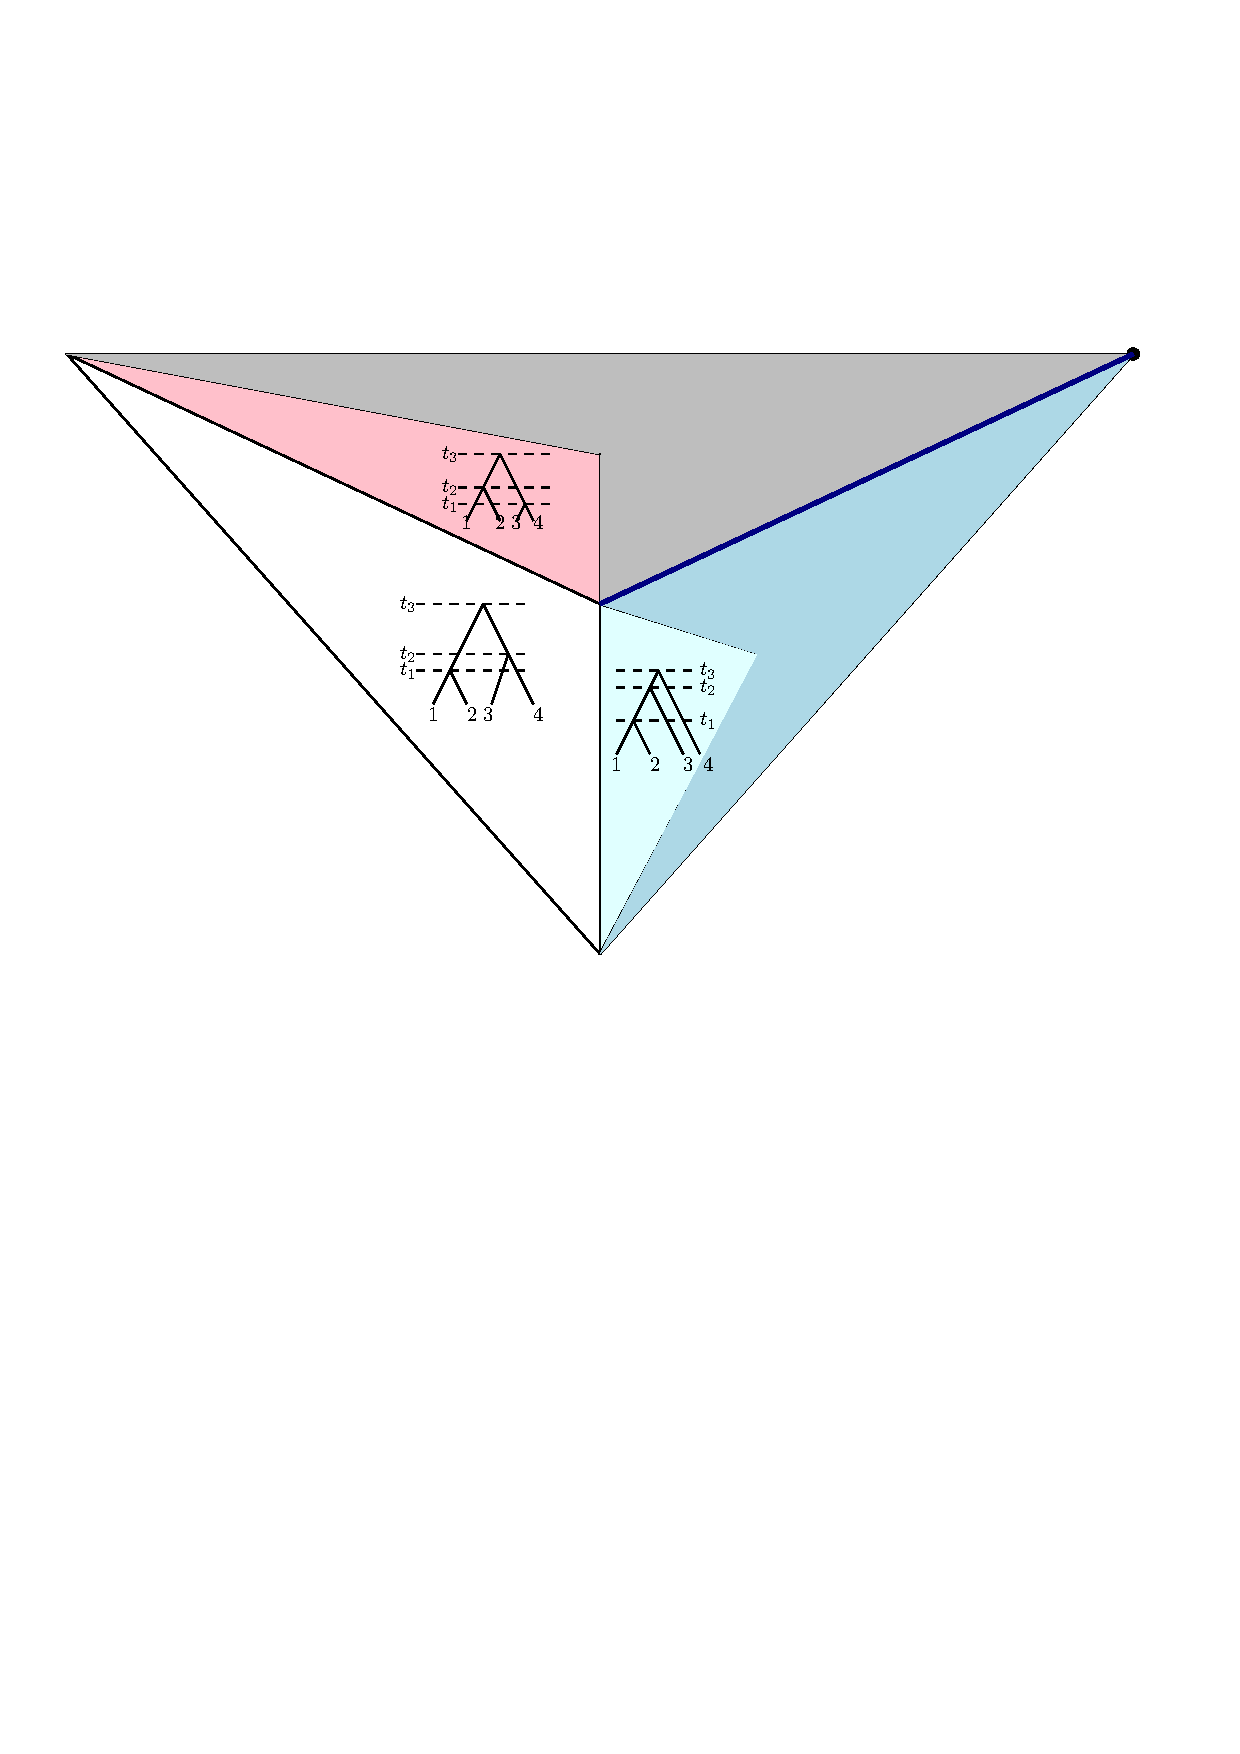
\includegraphics[width=\framewidth]{tSpace}
\end{definition}
\end{frame}

\begin{frame}{Motivation}
\begin{block}

\begin{enumerate}
\item Bayesian \MCMC: Mixing rate, access time, efficient proposals. 
\item Summarising posterior: No need to introduce several random variables on different probability spaces, no need to fit inconsistent data together. 
\item Interesting algorithmic/data structures problems: How to solve NP-complete problems on real computers for real data (Whidden and Matsen can compute \SPR-distance).
\item Interesting geometries: ``Every new example of a non-trivial simplicial complex of non-positive curvature is a big deal.''
\end{enumerate}
\end{block}
\end{frame}

\begin{frame}
Geodesic is a short for shortest path. 

\begin{theorem}[G and Drummond~\cite{Gavruskin2015}]
$\tau$-space has unique geodesics.
\end{theorem}

The reason this is true is pretty much the same as why this is true in \BHV space~\cite{bhv}. 

\begin{theorem}[G and Drummond~\cite{Gavruskin2015}]
Geodesics in $\tau$-space are efficiently computable. 
\end{theorem}

(Assuming $\mathcal O(n^4)$ is efficient.)

The reason this is true is pretty much the same as why this is true in \BHV space~\cite{owen2011fast}. 
\end{frame}

\begin{frame}{Nice metric spaces}
\begin{definition}
A metric space is called {\em nice} if most statisticians would like it. 
\end{definition}

Examples of nice metric spaces include real line, Euclidean space, and its nice subspaces. 

Examples of not nice metric spaces include all non-measurable subsets of a Euclidean space, all nowhere dense subsets of a Euclidean space, and most importantly the spaces where it is hard to define a random variable. 

\begin{theorem}[Billera, Holmes, and Vogtmann~\cite{bhv}]
The space of phylogenetic trees is a nice space. 
\end{theorem}

\begin{theorem}[G and Drummond~\cite{Gavruskin2015}]
The space of equidistant phylogenetic trees is a nice space. 
\end{theorem}
\end{frame}

\begin{frame}{Parameterisation matters!}
\begin{theorem}[G and Drummond~\cite{Gavruskin2015}]
\t-space is not a very nice space. 
\end{theorem}

That is,

\begin{theorem}[G and Drummond~\cite{Gavruskin2015}]
Geodesics in \t-space are hard to compute. Possible but hard. 
\end{theorem}

Hard here means that we (Alexei and I) don't know how. 
\end{frame}

\begin{frame}{By request only}
\begin{definition}
A geodesic metric space is called {\em nice} if it is a convex path-connected subspace of a computable metric space with unique geodesics of the same dimension. 
\end{definition}

\begin{theorem}[G and Drummond~\cite{Gavruskin2015}]
$\tau$-space is an efficiently computable cubical complex with unique geodesics. 
\end{theorem}

\begin{conjecture}[G and Drummond~\cite{Gavruskin2015}]
\t-space is a simplicial complex with unique geodesics, which are \NP-hard to compute. 
\end{conjecture}

\begin{corollary}
Both $\tau$-space and \t-space are nice.
\end{corollary}
\end{frame}



\begin{frame}{\href{http://alex.gavruskin.com/pictures/}{\Large{Thank you for your attention!}}}
\thebibliography{9}

\scriptsize

\bibitem{benner2014point}
Philipp Benner, Miroslav Ba{\v{c}}{\'a}k, and Pierre-Yves Bourguignon.
\newblock Point estimates in phylogenetic reconstructions.
\newblock {\em Bioinformatics}, 30(17):534--540, 2014.

\bibitem{bhv}
Louis~J Billera, Susan~P Holmes, and Karen Vogtmann.
\newblock Geometry of the space of phylogenetic trees.
\newblock {\em Advances in Applied Mathematics}, 27(4):733--767, 2001.

\bibitem{heled}
Joseph Heled and Remco~R Bouckaert.
\newblock Looking for trees in the forest: summary tree from posterior samples.
\newblock {\em BMC evolutionary biology}, 13(10):221, 2013.

\bibitem{hillis2005analysis}
David~M Hillis, Tracy~A Heath, and Katherine~St John.
\newblock Analysis and visualization of tree space.
\newblock {\em Systematic Biology}, 54(3):471--482, 2005.

\bibitem{owen2011fast}
Megan Owen and J~Scott Provan.
\newblock A fast algoritheorem for computing geodesic distances in tree space.
\newblock {\em IEEE/ACM Transactions on Computational Biology and
  Bioinformatics (TCBB)}, 8(1):2--13, 2011.

\bibitem{Gavruskin2015} Alex Gavryushkin and Alexei Drummond. 
\newblock The space of ultrametric phylogenetic trees. 
\newblock {\em arXiv preprint} \href{http://arxiv.org/abs/1410.3544}{arXiv:1410.3544}, 2014.
\end{frame}
\end{document}
